\documentclass[12pt,a4]{article}
\usepackage{physics, amsmath,amsfonts,amsthm,amssymb, mathtools,steinmetz, gensymb, siunitx}	% LOADS USEFUL MATH STUFF
\usepackage{xcolor,graphicx}
\usepackage{caption}
\usepackage{subcaption}
\usepackage[left=45pt, top=20pt, right=45pt, bottom=45pt ,a4paper]{geometry} 				% ADJUSTS PAGE
\usepackage{setspace}
\usepackage{tikz}
\usepackage{pdfpages}
\usepackage{pgf,tikz,pgfplots,wrapfig}
\usepackage{mathrsfs}
\usepackage{fancyhdr}
\usepackage{float}
\usepackage{array}
\usepackage{booktabs,multirow}
\usepackage{bm}
\usepackage{tensor}
\usepackage{listings}
 \lstset{
    basicstyle=\ttfamily\small,
    numberstyle=\footnotesize,
    numbers=left,
    backgroundcolor=\color{gray!10},
    frame=single,
    tabsize=2,
    rulecolor=\color{black!30},
    title=\lstname,
    escapeinside={\%*}{*)},
    breaklines=true,
    breakatwhitespace=true,
    framextopmargin=2pt,
    framexbottommargin=2pt,
    inputencoding=utf8,
    extendedchars=true,
    literate={á}{{$\rho$}}1 {ã}{{\~a}}1 {é}{{\'e}}1,
}
\DeclareMathOperator{\sign}{sgn}

\usetikzlibrary{decorations.text, calc}
\pgfplotsset{compat=1.7}

\usetikzlibrary{decorations.pathreplacing,decorations.markings}
\usepgfplotslibrary{fillbetween}

\newcommand{\vect}[1]{\boldsymbol{#1}}
\newcommand{\e}{\mathrm{d}}

\usepackage{hyperref}

%\usepackage[style= ACM-Reference-Format, maxbibnames=6, minnames=1,maxnames = 1]{biblatex}
%\addbibresource{references.bib}


\hypersetup{pdfborder={0 0 0},colorlinks=true,linkcolor=black,urlcolor=cyan,}
\allowdisplaybreaks
%\hypersetup{
%
%    colorlinks=true,
%
%    linkcolor=blue,
%
%    filecolor=magenta,      
%
%    urlcolor=cyan,
%
%    pdftitle={An Example},
%
%    pdfpagemode=FullScreen,
%
%    }
%}

\title{
\textsc{Gravitational Physics Homework 3}
}
\author{\textsc{J L Gouws}
}
\date{\today
\\[1cm]}



\usepackage{graphicx}
\usepackage{array}




\begin{document}
\thispagestyle{empty}

\maketitle

Acknowledgement: Many thanks go to PA for supplying me with Latex code for the figures which I modified slightly.\\
This homework might still be incomplete, but I have touched up some of my previous answers.
\begin{enumerate}
  \setcounter{enumi}{1}
  \item
    \begin{enumerate}
      \item
        Figure~\ref{fig:geodesicsOnplane} show two nearby geodesics (similar impact parameter) on the plane $\chi = \pi / 2$.
  \begin{figure}[H]
    \centering
    \begin{tikzpicture}[scale=2, rotate=0]
    
      % Define hyperbola parameters
      \def\a{1.2}
      \def\b{0.8}
      \def\c{-1}
    
      % Draw the hyperbola
      \draw[rotate=-18, dashed, red] plot[smooth,domain=-62:-19] ({\a*sec(\x)-2},{\b*tan(\x)});
      \draw[rotate=-28, dashed, red] plot[smooth,domain=-42:-22] ({1.5*\a*sec(\x-1) + \c -2},{2*\b*tan(\x-1)});
      \draw[rotate=-18] plot[smooth,domain=-19.5:72.7] ({\a*sec(\x)-2},{\b*tan(\x)});
      \draw[rotate=-28] plot[smooth,domain=-19:65.1] ({1.5*\a*sec(\x-1) + \c -2},{2*\b*tan(\x-1)});
      \draw[ultra thick] (0, 0) -- (-1.6, 0);
      \draw[rotate=-18, dashed] (0, 0) -- (-0.8, 0) node[left] {$r_0^1$};
      \draw[rotate=-28, dashed] (0, 0) -- (-1.5 * 0.8, 0) node[above left] {$r_0^2$};

%      \draw[rotate=-33, red] plot[smooth,domain=-28:54] ({1.5*\a*sec(\x-1) + \c -2.5},{2*\b*tan(\x-1)});

      \draw[rotate=-99, dashed, blue] (0, 0) -- (-1.6, 0) node[above left, black] {$r_{a,1}^1$};
      \draw[rotate=-128, dashed, blue] (0, 0) -- (-1.6, 0) node[above, black] {$r_{a,1}^2$};

      \draw[rotate=92, dashed, green] (0, 0) -- (-1.6, 0) node[below, black] {$r_{a,2}^1$};
      \draw[rotate=44, dashed, green] (0, 0) -- (-1.6, 0) node[below left, black] {$r_{a,2}^2$};

      \draw[->] (0, 0) -- (3, 1.05) node[right] {$\psi = 0$};
      \draw[fill=white, thick] (0,0) circle [radius=0.25];
      \draw[dashed] (0,0) circle [radius=1.6];


      \draw[rotate=-18] ({\a*sec(73)-2},{\b*tan(73)}) node {$1$};
      \draw[rotate=-28] ({1.5*\a*sec(66-1) + \c-2},{2*\b*tan(66-1)}) node {$2$};
      \draw (-1.6,0) node[above left] {$a$};
      \draw (-1.6/2,0) node[below left] {Disk};

      \draw[->] (3, 1.05) -- (-0.35*3+0.35*1.05 + 3, 3) node[right] {$b$};
      
      \draw (0,0) node {BH};
    \end{tikzpicture}
    \caption{Nearby Geodesics around blackhole}
    \label{fig:geodesicsOnplane}
  \end{figure}
  From the diagram we can see where the two geodesics meet the radius of the accretion disk $a$ and they intersect this at two points corresponding to two different partial deflection angles.
  \item
    Figure~\ref{fig:psiOfR} shows the total deflection angle as a function of the photon's radial distance.
  \begin{figure}[H]
    \centering
    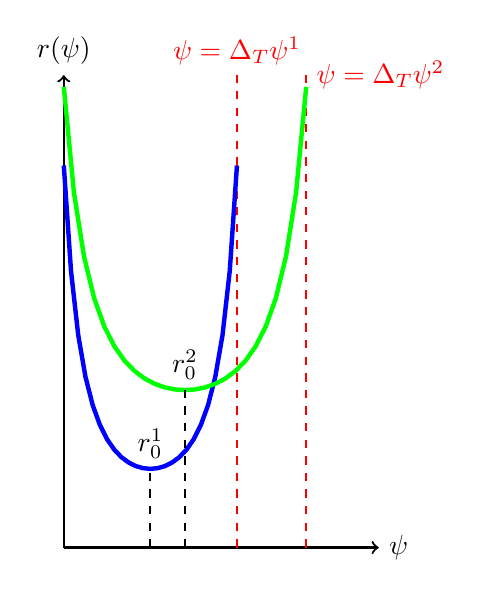
\begin{tikzpicture}[domain=-4:7] [scale=2]
      \draw[thick, ->] (0,0) -- (4,0) node[right] {$\psi$};
      \draw[thick,->] (0,0) -- (0,6) node[above] {$r(\psi)$}; %-
      \draw[thick, red, dashed] (.35*pi*2,0) -- (.35*pi*2,6) node[above] {$\psi = \Delta_T \psi^1$};
      \draw[thick, red, dashed] (.35*pi*2*1.4,0) -- (.35*pi*2*1.4, 6) node[right] {$\psi = \Delta_T \psi^2$};
%      \draw[thick, red, dashed] (0,0) -- (6,0) node[midway, below] {$\psi = 0$};
      \draw[ultra thick,color=blue] plot[domain=-.35*pi:.35*pi] (\x+0.35*pi, {1+tan(\x r)*tan(\x r)});
      \draw[ultra thick,color=green] plot[domain=-.35*pi:.35*pi] (1.4*\x+1.4*0.35*pi, {2+tan(\x r)*tan(\x r)});
      \draw[thick, dashed] (0.35*pi, 0) -- (0.35*pi, 1) node[above] {$r_0^1$};
      \draw[thick, dashed] (1.4*0.35*pi, 0) -- (1.4*0.35*pi, 2) node[above] {$r_0^2$};
    \end{tikzpicture}
    \caption{The deflection angle as a function of radial distance}
    \label{fig:psiOfR}
  \end{figure}

  \item 
  The figure below shows the deflection angle of the photon as a function of inverse radial distance.
  \begin{figure}[H]
    \centering
    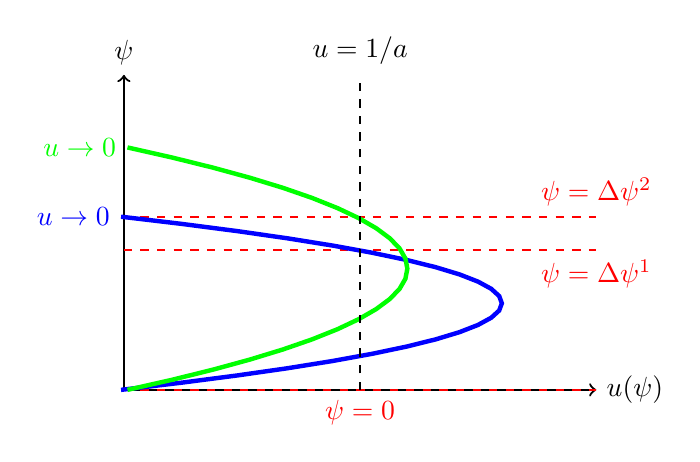
\begin{tikzpicture}[domain=-4:7] [scale=2]
      \draw[thick, ->] (0,0) -- (6,0) node[right] {$u(\psi)$};
      \draw[thick,->] (0,0) -- (0,4) node[above] {$\psi$};%-
      \draw[thick, red, dashed] (0,.35*pi*2) -- (6,.35*pi*2) node[pos=1, above] {$\psi = \Delta \psi^2$};
      \draw[thick, red, dashed] (0,.35*pi*2*1.4-1.3) -- (6,.35*pi*2*1.4-1.3) node[pos=1, below] {$\psi = \Delta \psi^1$};
      \draw[thick, red, dashed] (0,0) -- (6,0) node[midway, below] {$\psi = 0$};
      \draw[ultra thick,color=blue] plot[domain=-.35*pi:.35*pi] ({4*(0.2+1-\x*\x)}, \x+0.35*pi) node[left] {$u\to 0$};
      \draw[ultra thick,color=green] plot[domain=-.35*pi:.35*pi] ({1.5*(0.4+2-1.4*1.4*\x*\x)}, 1.4*\x+1.4*0.35*pi) node[left] {$u\to 0$};
      %\draw[thick, dashed] (0, 0.35*pi) -- (3*0.2+3, 0.35*pi) node[pos=0, left] {$u_0^1 = 1/r_0^1$};
      %\draw[thick, dashed] (0, 1.4*0.35*pi) -- (2.5*0.4+5, 1.4*0.35*pi) node[pos=0, left] {$u_0^2 = 1/r_0^2$};
      \draw[thick, dashed] (3, 0) -- (3, 4) node[pos=1, above] {$u = 1/a$};
    \end{tikzpicture}
    \caption{Deflection angle as a function of $1/r$}
    \label{fig:totalDeflection}
  \end{figure}
  The two branches come from whether the periastron is between the observer and the accretion disk or whether the periastron comes afterwards.
        
%        The below diagram shows two geodiesics emanating fron the accretion disc in parallel.
%        \begin{figure}[!ht]
%          \begin{center}
%            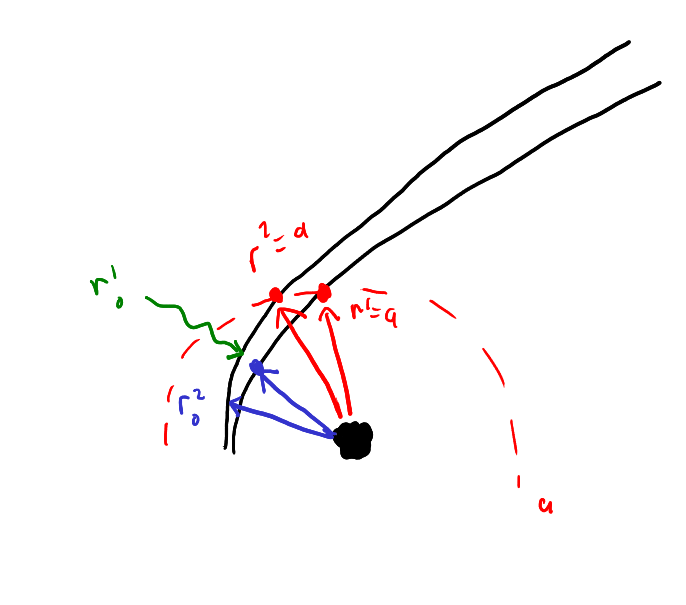
\includegraphics[scale=0.5]{ParallelGeodesics.png}
%          \end{center}
%          \caption{Parallel geodesics}
%        \end{figure}
    \end{enumerate}
  \item 
    \begin{enumerate}
      \setcounter{enumii}{1}
        \item
          The minimum size for the accretion disk is the size for which there can be stable matter orbits around the black whole, so that $a_{\min} = 6GM$.
      \setcounter{enumii}{4}
        \item
          The deflection angle comes from integrating along the path of the geodesic from $u = 0$ or $r = \infty$ up to some point.
    \end{enumerate}
  \item
    \begin{enumerate}
      \item
        The coordinates rotated by the angle $\theta_0$ are:
        \begin{align*}
          R_x(\theta_0) \mathbf{d} 
            &=  
                \left(
                \begin{matrix}
                  1 & 0 & 0\\
                  0 & \cos \theta_0 & -\sin \theta_0\\
                  0 & \sin \theta_0 & \cos \theta_0
                \end{matrix}
                \right)
                \left(
                \begin{matrix}
                  a \cos\phi' \\
                  a \sin \phi' \\
                  0 
                \end{matrix}
                \right)\\
            &= 
                \left(
                \begin{matrix}
                  a \cos\phi' \\
                  a \cos \phi_0 \sin \phi' \\
                  a \sin \phi_0 \sin \phi '
                \end{matrix}
                \right)
        \end{align*}
        And the observer's coordinates are:
        \begin{equation*}
          \left(
          \begin{matrix}
             a \sin \theta \cos \phi \\
             a \sin \theta \sin \phi \\
             a \cos \theta 
          \end{matrix}
          \right)
        \end{equation*}
        Equating the $z$ components gives:
        \begin{align*}
          \cos \theta = \sin \phi_0 \sin \phi' = \sin \phi_0 \frac{\sin \theta \sin \phi}{\cos \phi_0} & \Rightarrow \left(\tan \theta\right)^{-1} =  \tan \phi_0 \sin \phi\\
                                                                                                       & \Rightarrow \theta = \arctan\left(\frac{1}{\tan \phi_0 \sin \phi }\right)
        \end{align*}
        Equating the $x$ components gives:
        \begin{align*}
          \cos \phi' = \sin \theta \cos \phi = \frac{\cos \phi_0 \sin \phi'}{\sin \phi} \cos \phi & \Rightarrow \tan \phi ' =  \tan \phi \sec \theta_0\\
                                                                                                       & \Rightarrow \phi' = \arctan\left(\tan \phi \sec \theta_0\right)
        \end{align*}
    \end{enumerate}
  \item
    \begin{enumerate}
        \setcounter{enumii}{1}
      \item
        If we look at the accretion disk from directly above the shape is not distorted, but has radius slightly larger than the radius of the inner accretion disk, so we see a perfect circle which is the shape of the black hole.
        When the viewing angle increases, the accretion disk gets more and more squished and distorted.
    \end{enumerate}
\end{enumerate}
%\includepdf[pages=-]{gphw2Mathematica.pdf}
\end{document}
